\documentclass[11pt]{article}

\usepackage[margin=1in]{geometry}
\usepackage[T1]{fontenc}
\usepackage[utf8]{inputenc}
\usepackage{microtype}
\usepackage{amsmath}
\usepackage{amssymb}
\usepackage{booktabs}
\usepackage{graphicx}
\usepackage{hyperref}
\usepackage{array}
\usepackage{tabularx}
\usepackage{xcolor}
\usepackage[numbers,sort&compress]{natbib}

\hypersetup{
  colorlinks=true,
  linkcolor=blue!45!black,
  citecolor=blue!45!black,
  urlcolor=blue!45!black
}

\newcommand{\model}{FireWx-FM}
\newcommand{\grid}{5\,km}
\newcommand{\lead}{12-hour}
\newcolumntype{Y}{>{\raggedright\arraybackslash}X}

\title{\textbf{A Wildfire Foundation Model}}
\author{
  Yangshuang Xu \\
  Florida State University \\
  \texttt{yx21e@fsu.edu}
  \and
  Yuyang Dai \\
  Florida State University
  \and
  Liling Chang \\
  Florida State University
  \and
  Qi Wang \\
  Northeastern University
  \and
  Yushun Dong \\
  Florida State University
}
\date{}

\begin{document}
\maketitle

\begin{abstract}
\model{} is a wildfire-focused gridded model for short-lead active-fire occupancy prediction over the Lower 48 United States.
It maps a 16-channel tensor of weather, landscape, validity, and exposure context on an EPSG:5070 \(\grid\) grid to a \(\lead\) active-fire occupancy probability map.
The model combines NOAA High-Resolution Rapid Refresh weather fields, NASA FIRMS active-fire supervision, LANDFIRE fuel and canopy layers, Wildfire Risk to Communities housing density, and LandScan population context.
The architecture is a compact U-Net with 7.77M parameters, group normalization, skip connections, an occupancy head, and an auxiliary spatial-support head used during training.
The training recipe uses chronological splitting, train-split input normalization, sparse-label tile sampling, class-weighted binary cross-entropy, target dilation, and overlap-window inference for full-domain serving.
This report documents the model as a technical object: the data resources, input contract, target construction, architecture, training recipe, inference procedure, evaluation diagnostics, and intended use boundary.
\end{abstract}

\section{Introduction}

Wildfire prediction depends on a combination of fast-changing atmospheric conditions and slower landscape structure.
Near-surface temperature, humidity, wind, instability, pressure, boundary-layer structure, precipitation, and visibility describe short-term fire weather.
Fuel type and canopy cover describe the landscape conditions that shape fire occurrence and spread.
Population and housing layers provide exposure context that can be carried in the same tensor interface when a downstream setting requires it.
\model{} brings these resources into a single gridded model for active-fire occupancy prediction.

The task studied here is \emph{active-fire occupancy}.
Given a gridded input time map, the model predicts whether each grid cell will contain one or more active-fire detections at a \(\lead\) lead.
The output is a probability map on the same \(\grid\) grid.
Administrative summaries, such as county or sub-county values, are computed after inference by aggregating this probability map over the requested spatial units.
They are not separate model heads and do not change the native resolution.

We use the term foundation model in a scoped geospatial sense.
\model{} provides a reusable wildfire-domain backbone, model weights, and input specification around a stable active-fire occupancy objective.
Its scope is intentionally narrower than a general Earth-system model.
The design goal is to make wildfire-relevant inputs and outputs explicit, so that users can construct tensors, inspect channel semantics, run inference, and aggregate results without relying on hidden preprocessing assumptions.

This report follows the structure of a model technical report.
Section~\ref{sec:overview} summarizes the model.
Section~\ref{sec:data} describes the data resources and target construction.
Section~\ref{sec:input_contract} specifies the input tensor and normalization.
Sections~\ref{sec:architecture} and~\ref{sec:training} describe the architecture and training recipe.
Sections~\ref{sec:inference} and~\ref{sec:diagnostics} describe full-map inference and held-out diagnostics.
Section~\ref{sec:use_boundary} states the intended use boundary.

\section{Model Overview}
\label{sec:overview}

\model{} is a convolutional encoder-decoder model.
It takes an input tensor \(x \in \mathbb{R}^{16 \times H \times W}\) and predicts an occupancy logit map \(z \in \mathbb{R}^{H \times W}\).
The probability map is \(p=\sigma(z)\), where \(\sigma\) is the logistic sigmoid.
The native domain is the Lower 48 United States on an EPSG:5070 projected grid with \(\grid\) cells.

Table~\ref{tab:model_summary} gives the main model specification.
The model has one primary occupancy output.
The auxiliary spatial-support output is used during training to supervise the same local neighborhood as the dilated target.
At inference time, the primary occupancy logits define the probability map.

\begin{table}[t]
\centering
\small
\caption{Summary of the \model{} active-fire occupancy model.}
\label{tab:model_summary}
\begin{tabularx}{0.96\linewidth}{lY}
\toprule
Item & Specification \\
\midrule
Domain & Lower 48 United States \\
Native grid & EPSG:5070, \(\grid\) grid cells \\
Prediction target & Active-fire occupancy at a \(\lead\) lead \\
Input tensor & \(16\times H\times W\), channel-first order \\
Backbone & Compact U-Net with skip connections \\
Network normalization & Group normalization with up to 8 groups \\
Parameter count & 7.77M parameters with the auxiliary head included \\
Primary output & One occupancy logit per grid cell \\
Auxiliary output & Spatial-support logit used during training \\
Serving mode & Normalize continuous channels, then zero exposure channels 14 and 15 \\
Full-map inference & Overlap-window inference with phase averaging \\
\bottomrule
\end{tabularx}
\end{table}

The no-exposure serving mode keeps the 16-channel tensor interface while setting the housing-density and population channels to zero after normalization.
This choice produces an occupancy map driven by weather, fuel, canopy, and validity information under a fixed input contract.
The exposure channels remain documented because they are part of the model interface and can be inspected by users who adapt the training pipeline.

\section{Data Resources and Target Construction}
\label{sec:data}

\subsection{Dynamic Weather}

Dynamic weather inputs are derived from NOAA High-Resolution Rapid Refresh (HRRR) fields~\cite{noaa_hrrr_ncei,noaa_hrrr_emc}.
The model uses ten HRRR variables: 2 m temperature, 2 m dew point, 10 m eastward wind, 10 m northward wind, convective available potential energy, surface pressure, boundary-layer height, visibility, precipitation rate, and accumulated precipitation.
The CAPE channel is the HRRR 0--3000 m above-ground layer CAPE field.
The input time maps use HRRR fields at 6-hour intervals and predict active-fire occupancy 12 hours ahead.
All dynamic fields are placed on the common \(\grid\) EPSG:5070 grid.

\subsection{Active-Fire Supervision}

The supervised target is derived from NASA FIRMS active-fire detections~\cite{nasa_firms}.
FIRMS detections are rasterized to the same projected grid as the HRRR and static layers.
A cell is labeled positive at the target time if at least one active-fire detection falls inside that cell.
FIRMS is used as supervision rather than as an input channel.
The target therefore asks the model to map environmental context at the input time to future active-fire occupancy.

\subsection{Static Landscape and Exposure Context}

Static context provides information that does not change at the HRRR time step.
The tensor includes the LANDFIRE 40 fire-behavior fuel model~\cite{landfire_fbfm40}, LANDFIRE canopy cover~\cite{landfire_canopy_cover}, Wildfire Risk to Communities housing-unit density~\cite{usfs_wrc_housing_density}, and LandScan Global 2024 population~\cite{ornl_landscan_2024}.
The fire-behavior fuel model is a categorical code.
Canopy cover, housing density, and population are continuous channels.
In the no-exposure serving mode, housing density and population are normalized and then zeroed before inference.

\subsection{Grid Alignment and Validity}

All input layers are aligned to the same projected grid before tensors are built.
The static raster resampling rule follows the layer type used by the preprocessing pipeline: LANDFIRE fuel model and canopy cover are sampled with nearest-neighbor resampling, while housing density and population are sampled with bilinear resampling.
Two validity channels are included in the tensor.
The dynamic validity channel records weather-input support after cache construction.
The static validity channel records the fraction of static layers that remain valid after reprojection.
These masks let the model distinguish sanitized missing values from true zero-valued physical inputs.

\section{Input Contract}
\label{sec:input_contract}

\model{} expects channel-first tensors in \([16,H,W]\) order.
Channel order is part of the model definition.
Changing the order changes the meaning of the learned filters.
Table~\ref{tab:channels} specifies the complete channel contract.

\begin{table}[t]
\centering
\small
\caption{\model{} input channel contract.}
\label{tab:channels}
\begin{tabularx}{0.98\linewidth}{rlllY}
\toprule
Ch. & Name & Source & Unit & Description \\
\midrule
0 & \texttt{t2m} & HRRR & K & 2 m air temperature \\
1 & \texttt{d2m} & HRRR & K & 2 m dew point temperature \\
2 & \texttt{u10} & HRRR & m s\(^{-1}\) & 10 m eastward wind component \\
3 & \texttt{v10} & HRRR & m s\(^{-1}\) & 10 m northward wind component \\
4 & \texttt{cape} & HRRR & J kg\(^{-1}\) & CAPE, 0--3000 m above-ground layer \\
5 & \texttt{sp} & HRRR & Pa & Surface pressure \\
6 & \texttt{blh} & HRRR & m & Boundary-layer height \\
7 & \texttt{vis} & HRRR & m & Visibility \\
8 & \texttt{prate} & HRRR & kg m\(^{-2}\) s\(^{-1}\) & Precipitation rate \\
9 & \texttt{tp} & HRRR & kg m\(^{-2}\) & Accumulated precipitation \\
10 & \texttt{dynamic\_valid} & input builder & 0--1 & Dynamic weather validity fraction \\
11 & \texttt{static\_valid} & input builder & 0--1 & Static-layer validity fraction after reprojection \\
12 & \texttt{fuel\_fbfm40} & LANDFIRE & code & Fire-behavior fuel model \\
13 & \texttt{canopy\_cover} & LANDFIRE & percent & Canopy cover \\
14 & \texttt{housing\_density} & WRC & native & Housing-unit density; zeroed in no-exposure serving \\
15 & \texttt{population} & LandScan & persons & Population; zeroed in no-exposure serving \\
\bottomrule
\end{tabularx}
\end{table}

\subsection{Normalization}

Continuous channels are normalized with per-channel z-score statistics computed from the training split before tile sampling.
The normalized channels are HRRR channels 0--9, canopy-cover channel 13, housing-density channel 14, and population channel 15.
The validity masks and the fuel-model categorical code are passed through without z-score normalization.
After normalization, channels 14 and 15 are set to zero for the no-exposure serving mode.

This ordering matters.
Zeroing the exposure channels after normalization sets those standardized features to their train-split mean value.
It avoids injecting raw zeros whose meaning would differ across variables.
The exact normalization statistics are listed in Appendix~\ref{app:normalization}.

\subsection{Target}

The target \(y \in \{0,1\}^{H\times W}\) is a gridded occupancy map.
For each input time, the target time is 12 hours later.
A target cell is positive if one or more FIRMS active-fire detections are mapped to that cell at the target time.
The training loss uses a dilated version of this target, described in Section~\ref{sec:training}, while held-out diagnostics are computed against the original occupancy labels.

\section{Architecture}
\label{sec:architecture}

\model{} uses a compact U-Net architecture~\cite{ronneberger2015unet}.
The encoder has four downsampling stages and a bottleneck.
Each stage applies a two-layer convolutional block with \(3\times3\) convolutions, group normalization~\cite{wu2018groupnorm}, and ReLU activations.
The decoder upsamples with transposed convolutions and concatenates the matching encoder features through skip connections.
The base width is 32 channels.
The bottleneck width is 512 channels.

The model has two \(1\times1\) output heads.
The primary head predicts active-fire occupancy logits.
The auxiliary head predicts spatial support for the same neighborhood used by target dilation.
Dropout with rate 0.1 is applied before the heads.
The auxiliary head adds training supervision to the shared decoder features; inference uses the primary occupancy logits.

The model is fully convolutional.
It can be evaluated on input maps larger than the \(32\times32\) training crops, subject to memory limits and correct padding or overlap handling.
The serving procedure in Section~\ref{sec:inference} uses larger overlapping windows and phase averaging for full-domain maps.

\section{Training Recipe}
\label{sec:training}

\subsection{Chronological Split}

Training uses a chronological split over 2024 time maps.
June--August 2024 are used for training.
September 2024 is used for validation.
The October 2024 evaluation window is held out for testing.
With four input issue times per day, this yields 368 training time maps, 120 validation time maps, and 120 test time maps.
Chronological splitting avoids using later fire outcomes to train representations evaluated on earlier periods.

\subsection{Sparse-Label Tile Sampling}

Active-fire occupancy is rare at \(\grid\) resolution.
Training therefore samples \(32\times32\) crops from the full time maps.
Positive crops are selected so that active-fire cells are contained somewhere in the crop, rather than always placed at a fixed center location.
Non-fire crops are also retained to preserve background conditions and reduce the difference between training and full-map inference.
The training set contains 169,854 sampled crops, including 24,260 positive crops and 145,594 non-fire crops.

The \(32\times32\) crop size is a training-sampling choice.
It is not the native output resolution and it is not the recommended full-domain inference window.
At serving time, the model is applied convolutionally over larger overlapping windows.

\subsection{Objective}

The primary objective is binary cross-entropy on the active-fire occupancy target with positive-class weighting.
The positive weight used in the run documented here is 10.
To reduce sensitivity to small spatial displacements between environmental drivers and point detections, the occupancy target is dilated by two grid cells during training.
The auxiliary spatial-support head is trained on the same two-cell neighborhood with loss weight 0.5.

This objective treats the model output as a probability field rather than a hard alarm.
Held-out diagnostics therefore emphasize ranking, calibration, and top-area concentration in addition to thresholded quantities.

\subsection{Optimization}

The model is trained with AdamW~\cite{loshchilov2019adamw}.
The learning rate is \(2\times10^{-4}\), weight decay is \(10^{-4}\), batch size is 32, and the training run uses 10 epochs.
The output-head bias is initialized from the training positive rate.
Horizontal and vertical flips are used as crop-level augmentation.
Mixed precision is used when available.
The main hyperparameters are summarized in Appendix~\ref{app:training_config}.

\section{Full-Map Inference}
\label{sec:inference}

\subsection{Serving Steps}

Inference starts from a 16-channel tensor on the native grid.
Continuous channels are normalized using the train-split statistics.
Channels 14 and 15 are then set to zero for no-exposure serving.
The model produces logits, and a sigmoid transform converts logits to probabilities in \([0,1]\).
The output map has shape \([H,W]\) and shares the grid with the input tensor.

\subsection{Overlap-Window Prediction}

Full-domain inference uses overlapping windows rather than independent \(32\times32\) crops.
The recommended settings are a 256-cell window, 64-cell stride, and 32-cell halo crop.
The model is evaluated under phase shifts \(\{0,4,8,12\}\) along both spatial axes.
Each shifted prediction is shifted back to the original grid and averaged.
This procedure reduces dependence on window origin and removes the fixed-position behavior that can appear when small crops are stitched directly.

\subsection{Spatial Aggregation}

The native output is a gridded probability map.
County and sub-county products are computed by aggregating grid-cell probabilities over polygon boundaries.
Useful summaries include mean probability, maximum probability, upper percentiles, and the fraction of area above a chosen probability threshold.
These summaries are transparent post-inference operations.
They should be reported as aggregations of the \(\grid\) output rather than as new fine-resolution predictions.

\begin{figure}[t]
\centering
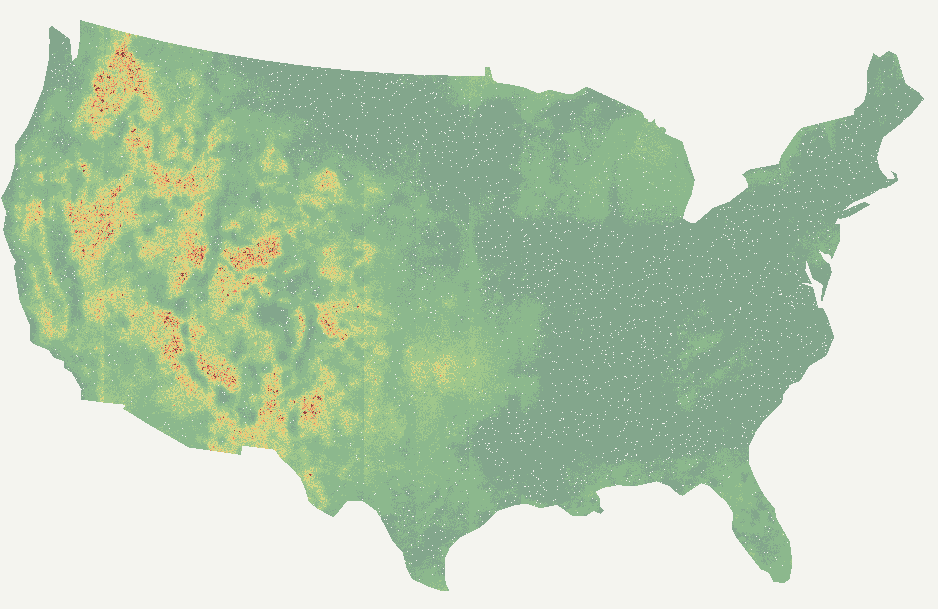
\includegraphics[width=0.92\linewidth]{figures/firewxfm_conus_20260706_t12_usgs_calibrated_heatmap.png}
\caption{Example \model{} active-fire occupancy overlay generated from 2026-07-06 12:00 UTC HRRR input, with a 12-hour lead to 2026-07-07 00:00 UTC. The example applies USGS-consistency calibration using same-day USGS Fire Danger Forecast surfaces~\cite{usgs_fire_danger_forecast}. The rendered image uses a green-dominant discrete speckled raster display: cell-level categorical marks, deterministic micro-texture, fragmented warm-color pockets, and no Gaussian blur or smooth interpolation. Quantitative analysis should use the probability raster.}
\label{fig:example_heatmap}
\end{figure}

\section{Diagnostics}
\label{sec:diagnostics}

Table~\ref{tab:diagnostics} reports held-out diagnostics on the October 2024 evaluation window.
The active-fire label is extremely sparse, so absolute precision and PR-AUC values are small.
Top-area recall and lift describe whether active-fire cells are concentrated in high-scoring regions of the map.
These diagnostics characterize the probability field for the occupancy task.
They are not deployment thresholds.

\begin{table}[t]
\centering
\small
\caption{Held-out diagnostics for \model{} active-fire occupancy prediction.}
\label{tab:diagnostics}
\begin{tabular}{lc}
\toprule
Diagnostic & Value \\
\midrule
PR-AUC & 0.000721 \\
AUROC & 0.7466 \\
Brier score & 0.000198 \\
Expected calibration error & 0.00485 \\
Top 0.1\% precision & 0.00489 \\
Top 0.1\% recall & 0.0332 \\
Top 0.1\% lift & 33.24 \\
Top 1\% precision & 0.00150 \\
Top 1\% recall & 0.1017 \\
Top 1\% lift & 10.17 \\
Top 10\% recall & 0.2951 \\
Top 10\% lift & 2.95 \\
\bottomrule
\end{tabular}
\end{table}

The example 2026-07-06 12:00 UTC probability raster has grid shape \(609\times938\).
It predicts active-fire occupancy at a 12-hour lead, corresponding to 2026-07-07 00:00 UTC.
For the public example, the raw model map is post-processed with a USGS-consistency calibration that blends the smoothed model rank with USGS WFPI, large-fire-probability, and fire-spread-probability ranks for 2026-07-07.
Inside the Lower-48 mask, the calibrated mean probability is 0.0367.
The maximum probability in the masked raster is 0.3353.
The 99th and 99.9th percentiles of the masked raster are 0.1782 and 0.2612.
These values describe one input time map and should not be interpreted as climatological frequencies.
The rendered preview in Figure~\ref{fig:example_heatmap} uses a display-only discrete speckled raster transform.
It converts the calibrated probability field into small categorical cell marks with deterministic jitter, micro-clusters, short streaks, fragmented edges, and a green-to-yellow-to-orange-to-red wildfire-risk palette.
This rendering makes low-probability regional structure, including eastern U.S. spatial variation, visible in the preview without turning the map into a smooth continuous heatmap; it does not change the probability raster.
The eastern U.S. is not masked or missing in the input stack.
Diagnostic checks show valid dynamic weather support and static-layer support over the region, while the raw model assigns much lower active-fire occupancy scores east of the Mississippi than in the western U.S. for this example date.

\section{Use Boundary}
\label{sec:use_boundary}

\model{} is intended for research and screening use in gridded active-fire occupancy prediction.
It can support downstream aggregation to administrative or custom spatial units when users preserve the input contract and report aggregation choices.
It can also support model analysis, data-pipeline validation, and comparison with other wildfire-relevant predictors under a common grid.

The model is not an emergency-response system.
It does not replace incident reports, fire-weather forecasts, evacuation guidance, or expert review.
Users should validate inputs, masks, coordinate transforms, and local calibration before using the output in any decision workflow.
Raw source datasets are not redistributed with the model.
Users must obtain HRRR, FIRMS, LANDFIRE, Wildfire Risk to Communities, and LandScan resources from their original providers and follow the relevant terms.

\section{Conclusion}

\model{} defines a wildfire-domain foundation model around a concrete active-fire occupancy task.
Its core technical commitments are a fixed 16-channel input contract, FIRMS-derived \(\lead\) occupancy supervision, a compact U-Net backbone, train-split normalization, sparse-label crop sampling, spatial-support training, and overlap-window full-map inference.
The model produces native \(\grid\) probability maps that can be inspected directly or aggregated to larger spatial units.
By documenting the data sources, channel semantics, target construction, and inference procedure, the report makes the model usable as a transparent building block for wildfire-focused geospatial modeling.

\bibliographystyle{plainnat}
\bibliography{reference_tech}

\appendix

\section{Training Configuration}
\label{app:training_config}

\begin{table}[h]
\centering
\small
\caption{Main training configuration.}
\label{tab:training_config}
\begin{tabular}{ll}
\toprule
Item & Value \\
\midrule
Input channels & 16 \\
Native grid & Lower-48 United States, EPSG:5070, \(\grid\) \\
Lead time & 12 hours \\
Training period & June--August 2024 \\
Validation period & September 2024 \\
Test window & October 2024 \\
Input issue times & 00, 06, 12, and 18 UTC \\
Training time maps & 368 \\
Validation time maps & 120 \\
Test time maps & 120 \\
Crop size & \(32\times32\) cells \\
Training crops & 169,854 \\
Positive crops & 24,260 \\
Non-fire crops & 145,594 \\
Base channels & 32 \\
Network normalization & Group normalization \\
Dropout & 0.1 \\
Loss & Class-weighted binary cross-entropy \\
Positive weight & 10 \\
Target dilation & 2 grid cells \\
Auxiliary spatial loss weight & 0.5 \\
Optimizer & AdamW \\
Learning rate & \(2\times10^{-4}\) \\
Weight decay & \(10^{-4}\) \\
Batch size & 32 \\
Epochs & 10 \\
\bottomrule
\end{tabular}
\end{table}

\section{Input Normalization Statistics}
\label{app:normalization}

\begin{table}[h]
\centering
\small
\caption{Train-split z-score statistics for normalized channels.}
\label{tab:normalization}
\begin{tabular}{rllrr}
\toprule
Ch. & Name & Unit & Mean & Std. \\
\midrule
0 & \texttt{t2m} & K & 295.5830 & 6.5945 \\
1 & \texttt{d2m} & K & 288.8014 & 7.6761 \\
2 & \texttt{u10} & m s\(^{-1}\) & -0.1179 & 3.2024 \\
3 & \texttt{v10} & m s\(^{-1}\) & 0.0219 & 3.9899 \\
4 & \texttt{cape} & J kg\(^{-1}\) & 747.1428 & 1110.3022 \\
5 & \texttt{sp} & Pa & 96817.9246 & 6815.0126 \\
6 & \texttt{blh} & m & 681.3271 & 684.6619 \\
7 & \texttt{vis} & m & 26947.7353 & 20073.7663 \\
8 & \texttt{prate} & kg m\(^{-2}\) s\(^{-1}\) & 0.0000 & \(10^{-6}\) \\
9 & \texttt{tp} & kg m\(^{-2}\) & 0.0000 & \(10^{-6}\) \\
13 & \texttt{canopy\_cover} & percent & 8.2556 & 21.4576 \\
14 & \texttt{housing\_density} & native & 7.2324 & 62.6264 \\
15 & \texttt{population} & persons & 14.2284 & 122.3255 \\
\bottomrule
\end{tabular}
\end{table}

\section{Public Artifacts}
\label{app:artifacts}

\begin{table}[h]
\centering
\small
\caption{Primary artifacts associated with the model report.}
\label{tab:artifacts}
\begin{tabularx}{0.98\linewidth}{lY}
\toprule
Artifact & Purpose \\
\midrule
Model weights & Store the learned U-Net parameters for active-fire occupancy prediction. \\
Input-channel metadata & Records channel order, source dataset, unit, and variable description. \\
Normalization statistics & Records train-split z-score statistics for continuous input channels. \\
Inference code & Applies normalization, no-exposure serving, overlap-window prediction, and phase averaging. \\
Training code & Documents cache construction, sparse-label crop sampling, objective functions, and optimization. \\
Example probability raster & Provides a quantitative \(\grid\) probability output for one CONUS time map. \\
Rendered heatmap & Provides a discrete speckled raster preview of the same probability output. \\
Data-source notes & Point users to the original data providers; raw source data are not redistributed. \\
\bottomrule
\end{tabularx}
\end{table}

\end{document}
